\part{Synchronous machine}
\title[Synchronous machine]{Synchronous machine}  
\date{}  
\frame{\titlepage} 

%%%%%%%%%%%%%%%%%%%%%%%%%%%%%%%%%%%%%%%%%%%%%%%%%%%%%%%%%%%%%
%% Synchronous machine (SM) rotor types %%
%%%%%%%%%%%%%%%%%%%%%%%%%%%%%%%%%%%%%%%%%%%%%%%%%%%%%%%%%%%%%
\begin{frame}
	\frametitle{Synchronous machine (SM) rotor types}
	\begin{figure}
		\centering
		\begin{subfigure}{0.49\textwidth}
			\centering
			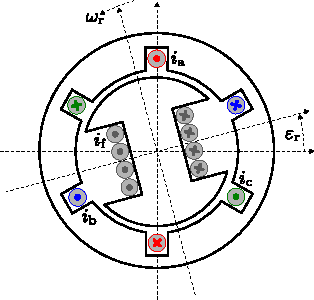
\includegraphics[width=0.8\textwidth]{fig/lec07/SM_salient_pole.pdf}
			\caption{Salient pole rotor}
		\end{subfigure}
		\hfill
		\begin{subfigure}{0.49\textwidth}
			\centering
			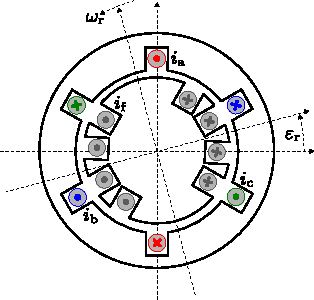
\includegraphics[width=0.8\textwidth]{fig/lec07/SM_cylindrical_rotor.pdf}
			\caption{Cylindrical rotor}
		\end{subfigure}
        \caption{Major rotor types of synchronous machines (SM)} 
        \label{fig:examples_SM_rotor}
	\end{figure}
\end{frame}

%%%%%%%%%%%%%%%%%%%%%%%%%%%%%%%%%%%%%%%%%%%%%%%%%%%%%%%%%%%%%
%% SM application examples %%
%%%%%%%%%%%%%%%%%%%%%%%%%%%%%%%%%%%%%%%%%%%%%%%%%%%%%%%%%%%%%
\begin{frame}
	\frametitle{SM application examples}
	\begin{figure}
		\centering
		\begin{subfigure}{0.49\textwidth}
			\centering
			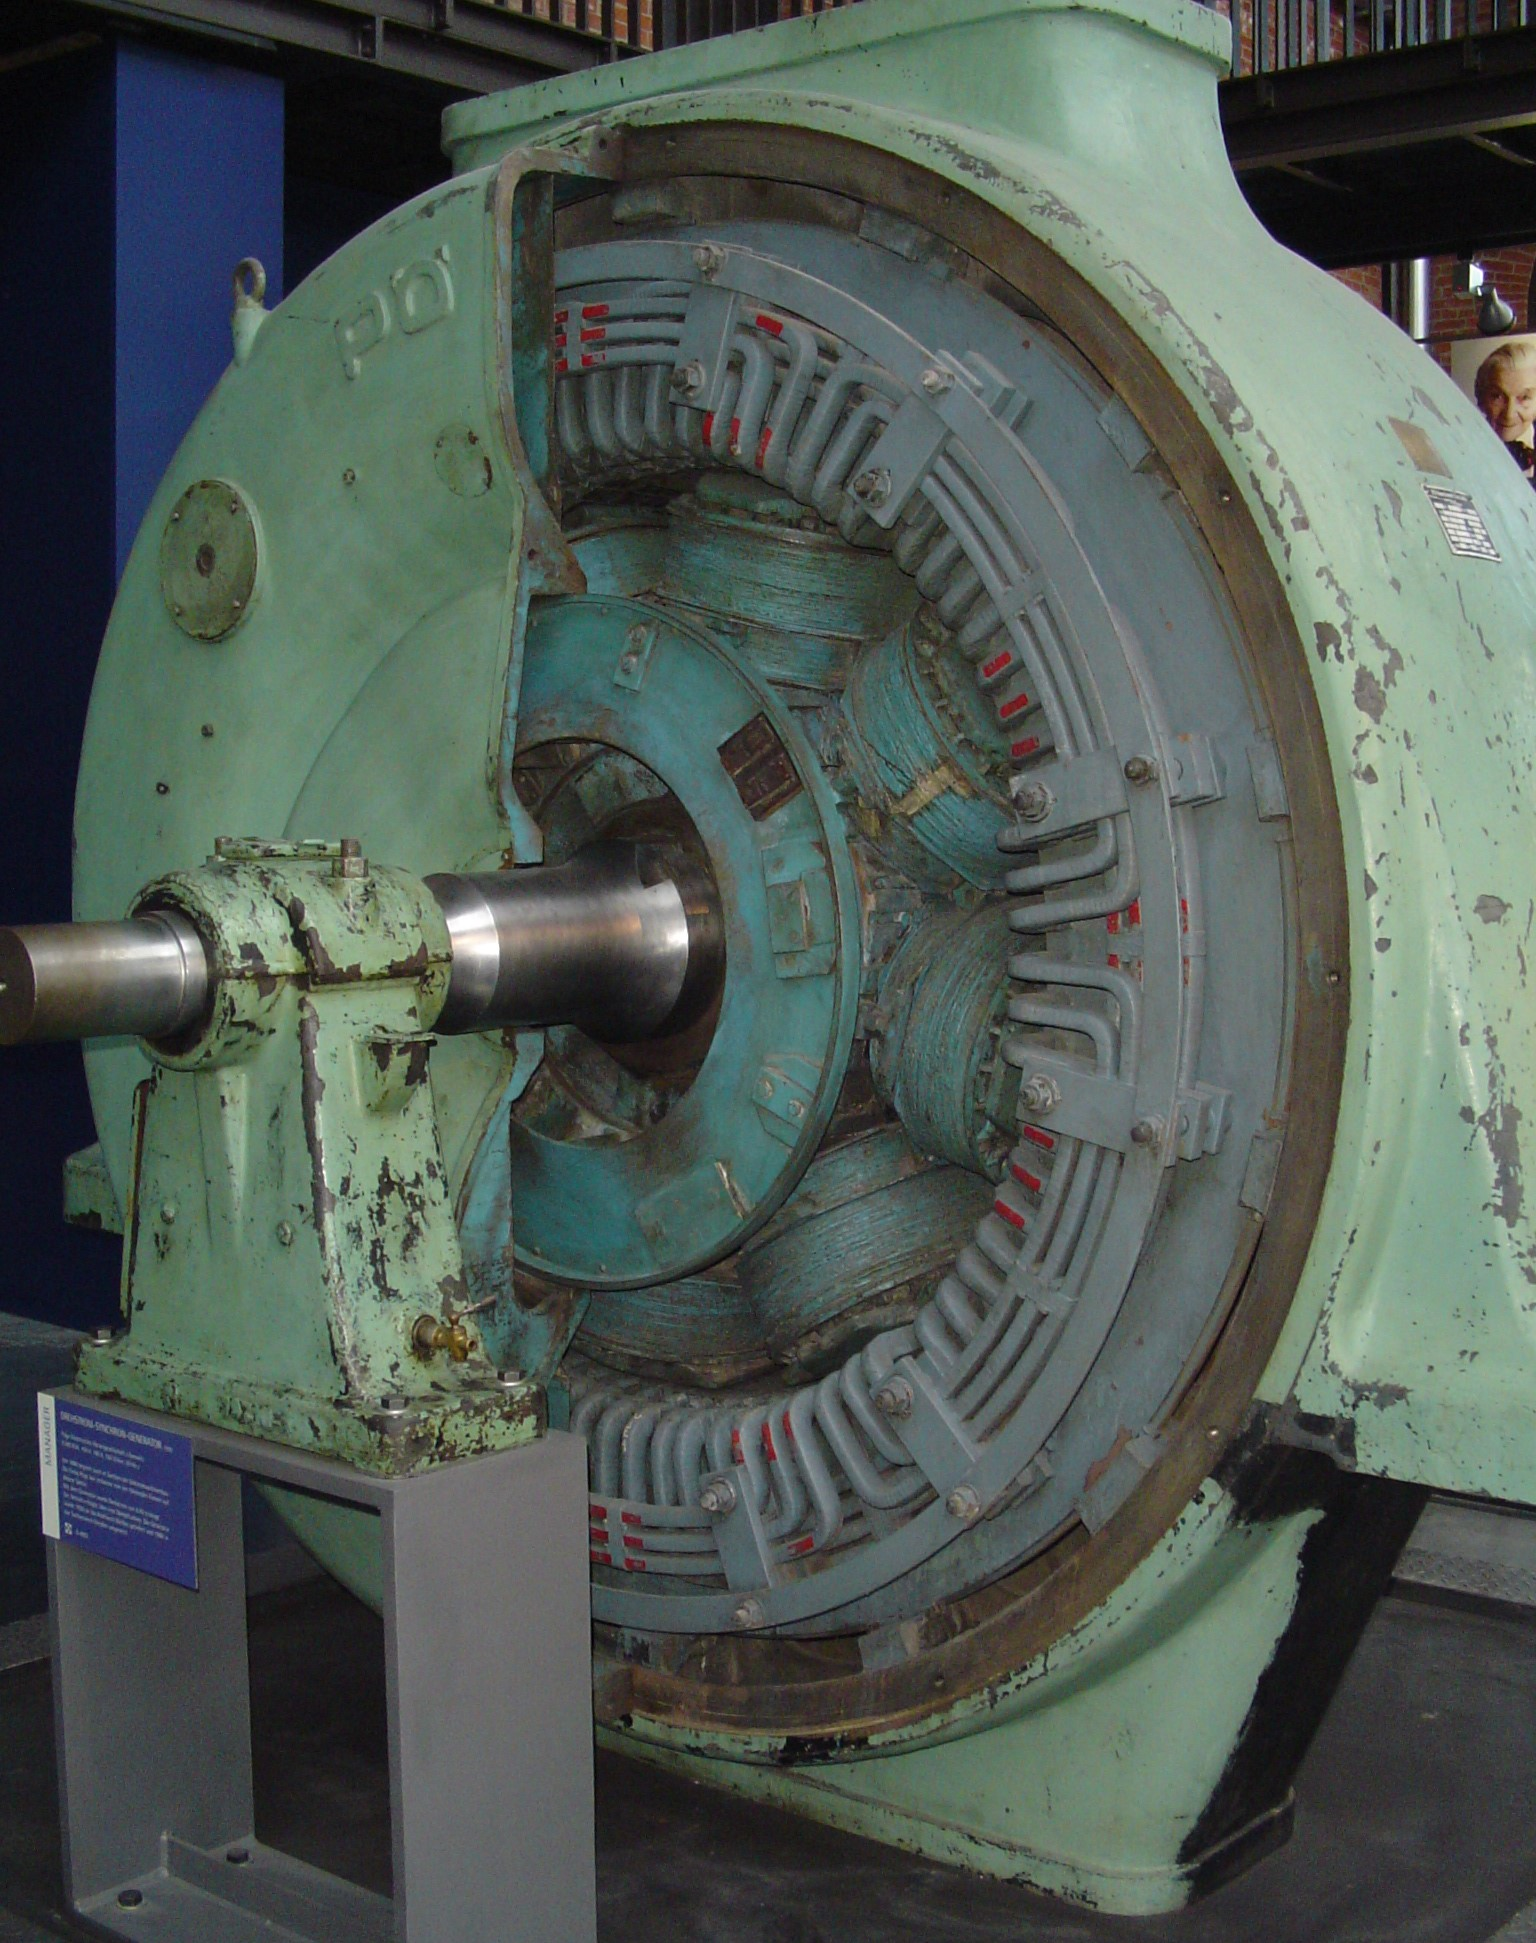
\includegraphics[height=0.55\textheight]{fig/lec07/Salient_pole_rotor.jpg}
			\caption{\SI{2}{\mega\volt\ampere} generator from 1920 (source: \href{hhttps://commons.wikimedia.org/wiki/File:Drehstrom-Synchron-Generator.jpg}{Wikimedia Commons}, Kolossos, \href{https://creativecommons.org/licenses/by-sa/3.0/deed}{CC BY-SA 3.0})}
		\end{subfigure}
		\hfill
		\begin{subfigure}{0.49\textwidth}
			\centering
			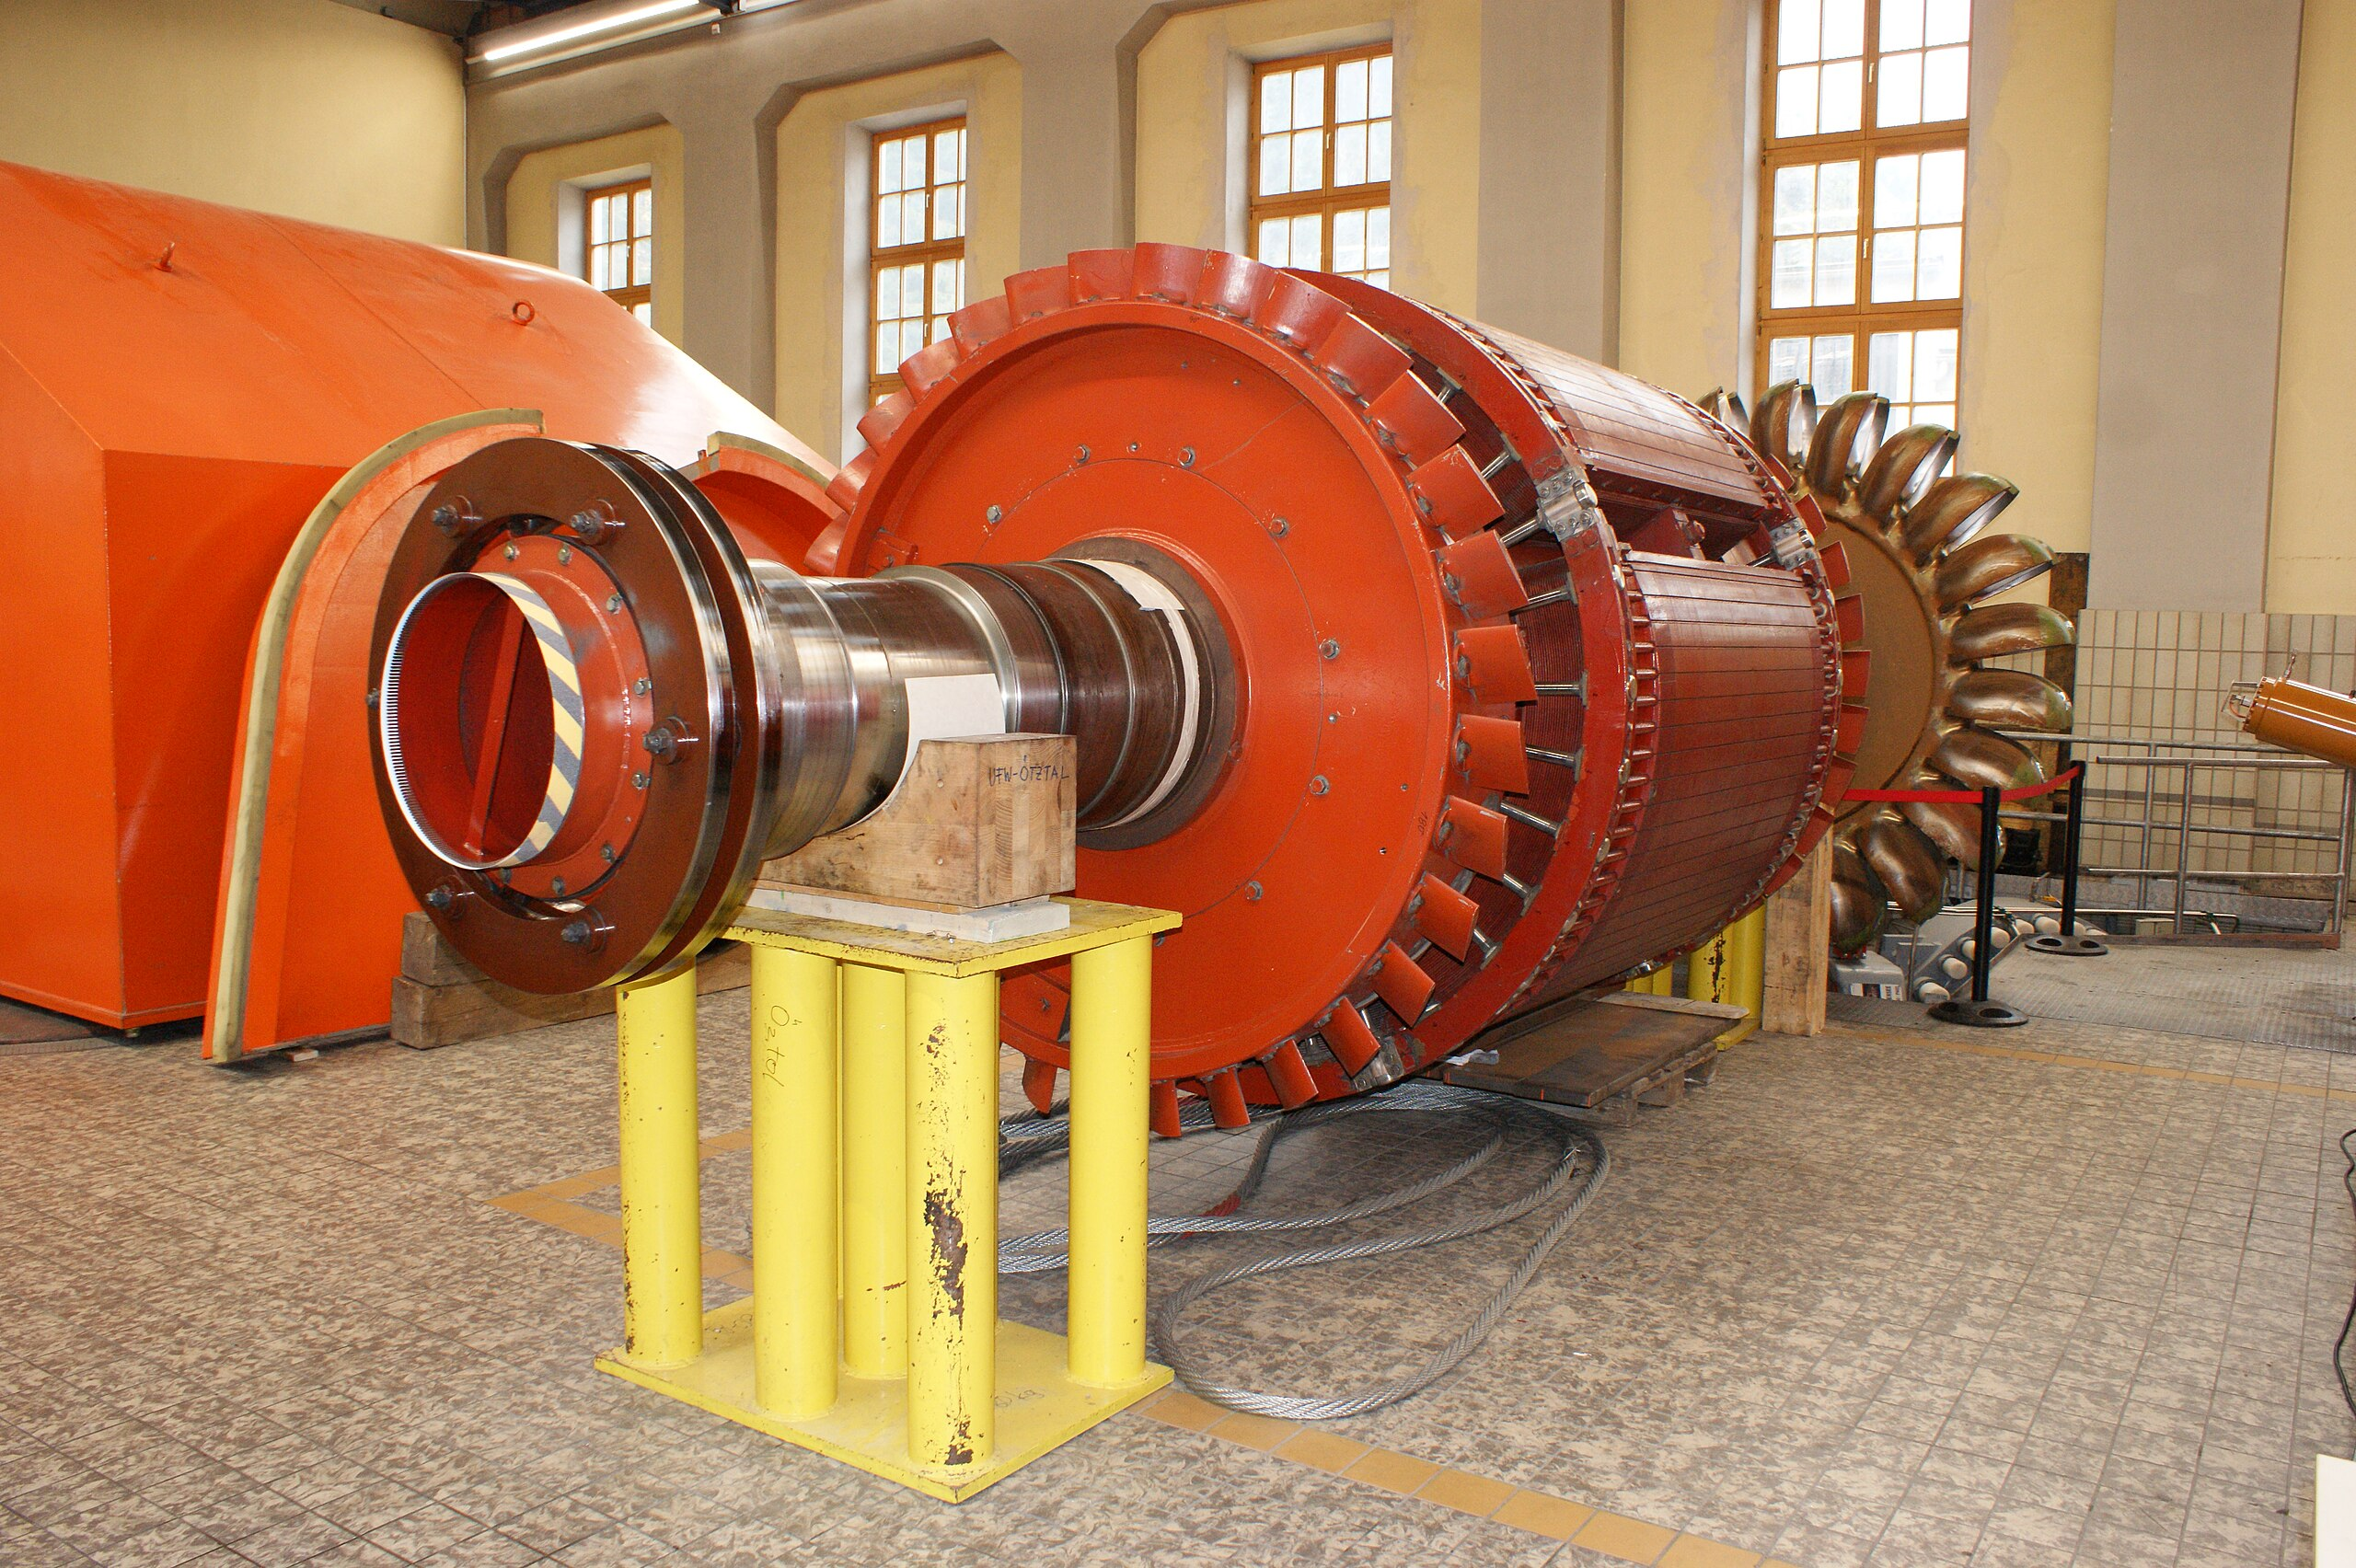
\includegraphics[height=0.55\textheight]{fig/lec07/Pelton_wheel_rotor.jpg}
			\caption{\SI[tight-spacing=true]{36}{\mega\volt\ampere} Pelton wheel generator (source: \href{https://commons.wikimedia.org/wiki/File:Wald_am_Arlberg-OeBB_Spullersee_power_plant-M1-Rotor-09ASD.jpg}{Wikimedia Commons},  	Asurnipal, \href{https://creativecommons.org/licenses/by-sa/4.0/deed}{CC BY-SA 4.0})} 
		\end{subfigure}
        \caption{SM examples with salient pole rotor type} 
        \label{fig:examples_SM_applications_01}
	\end{figure}
\end{frame}

%%%%%%%%%%%%%%%%%%%%%%%%%%%%%%%%%%%%%%%%%%%%%%%%%%%%%%%%%%%%%
%% SM application examples (cont.) %%
%%%%%%%%%%%%%%%%%%%%%%%%%%%%%%%%%%%%%%%%%%%%%%%%%%%%%%%%%%%%%
\begin{frame}
	\frametitle{SM application examples (cont.)}
	\begin{figure}
		\centering
		\begin{subfigure}{0.49\textwidth}
			\centering
			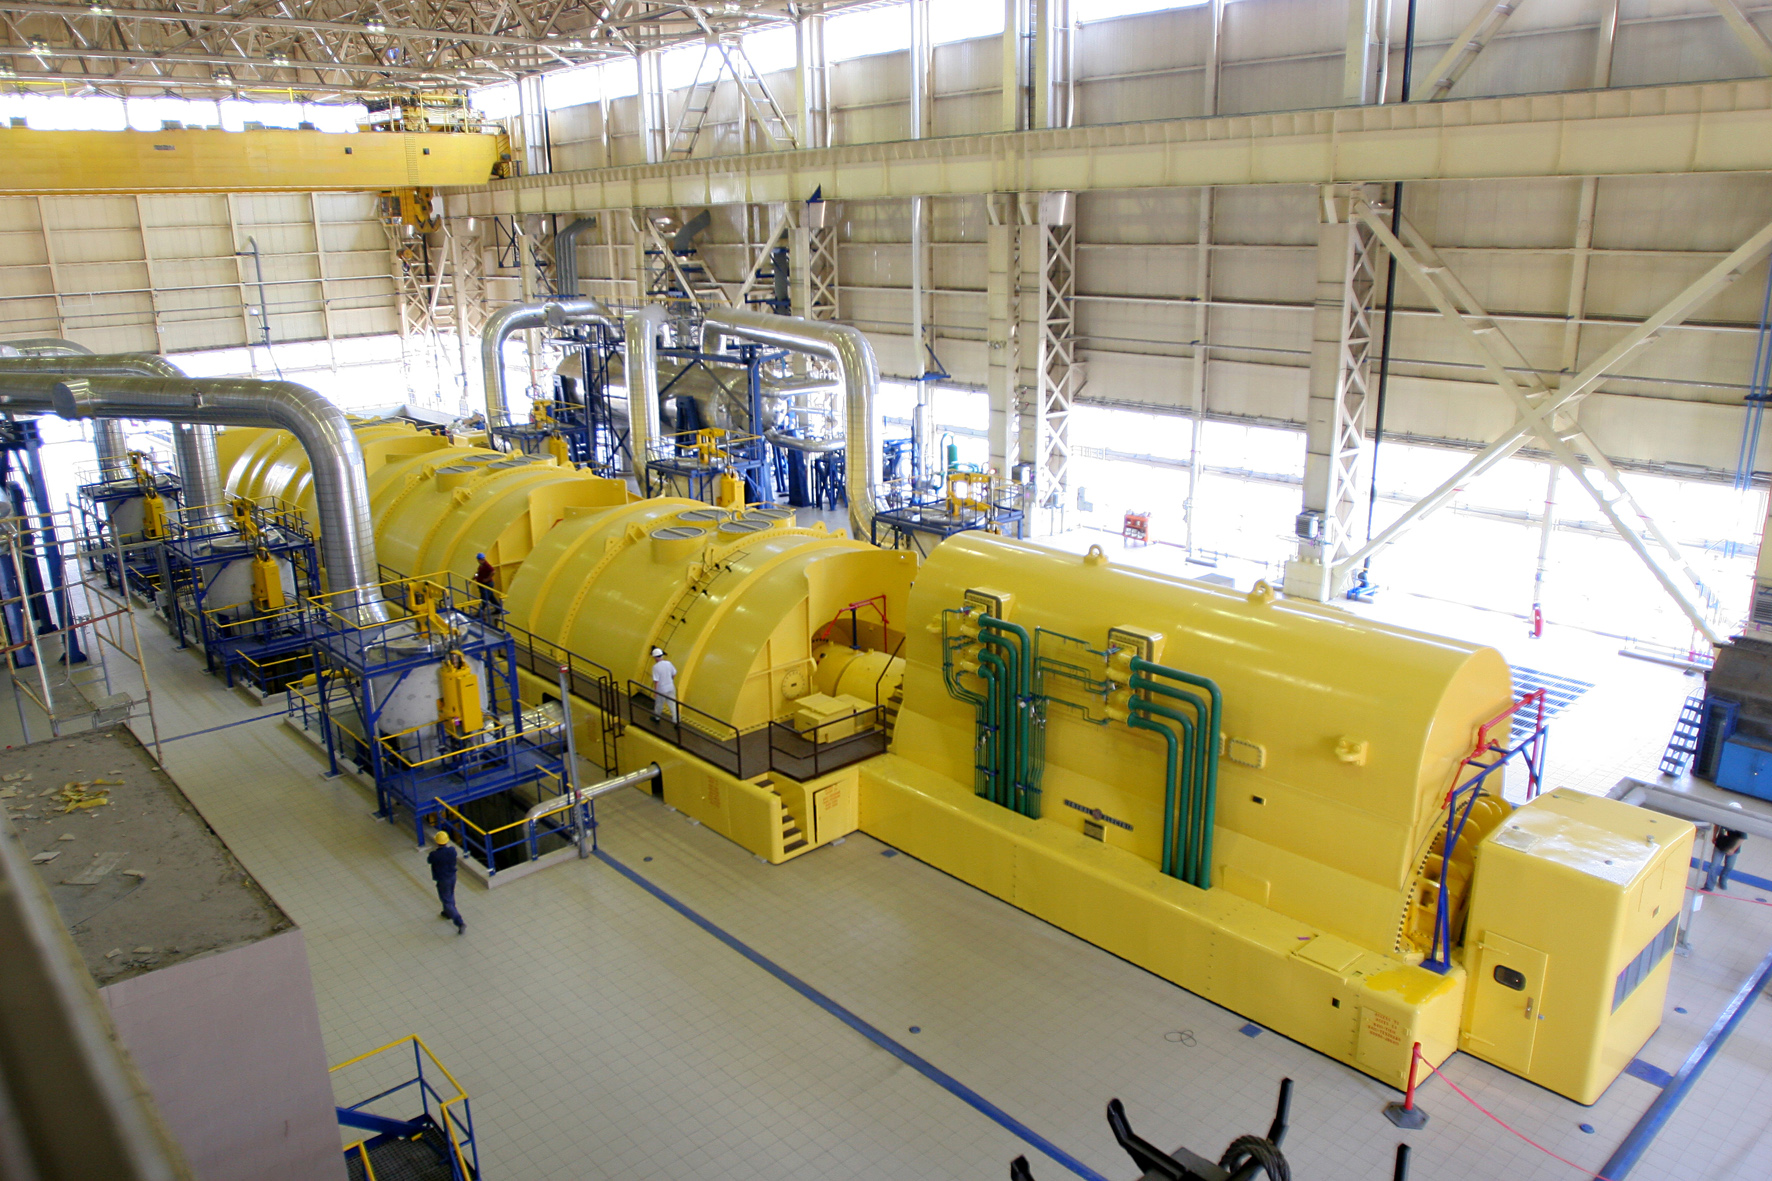
\includegraphics[height=0.55\textheight]{fig/lec07/Turbogenerator.jpg}
			\caption{\SI{650}{\mega\volt\ampere} turbogenerator from Cernavodă nuclear power plant (source: \href{https://commons.wikimedia.org/wiki/File:Grupul_turbogenerator_CNE_Cernavoda.jpg}{Wikimedia Commons}, R. Lavinia, \href{https://creativecommons.org/licenses/by-sa/4.0/deed}{CC BY-SA 4.0})}
		\end{subfigure}
		\hfill
		\begin{subfigure}{0.49\textwidth}
			\centering
			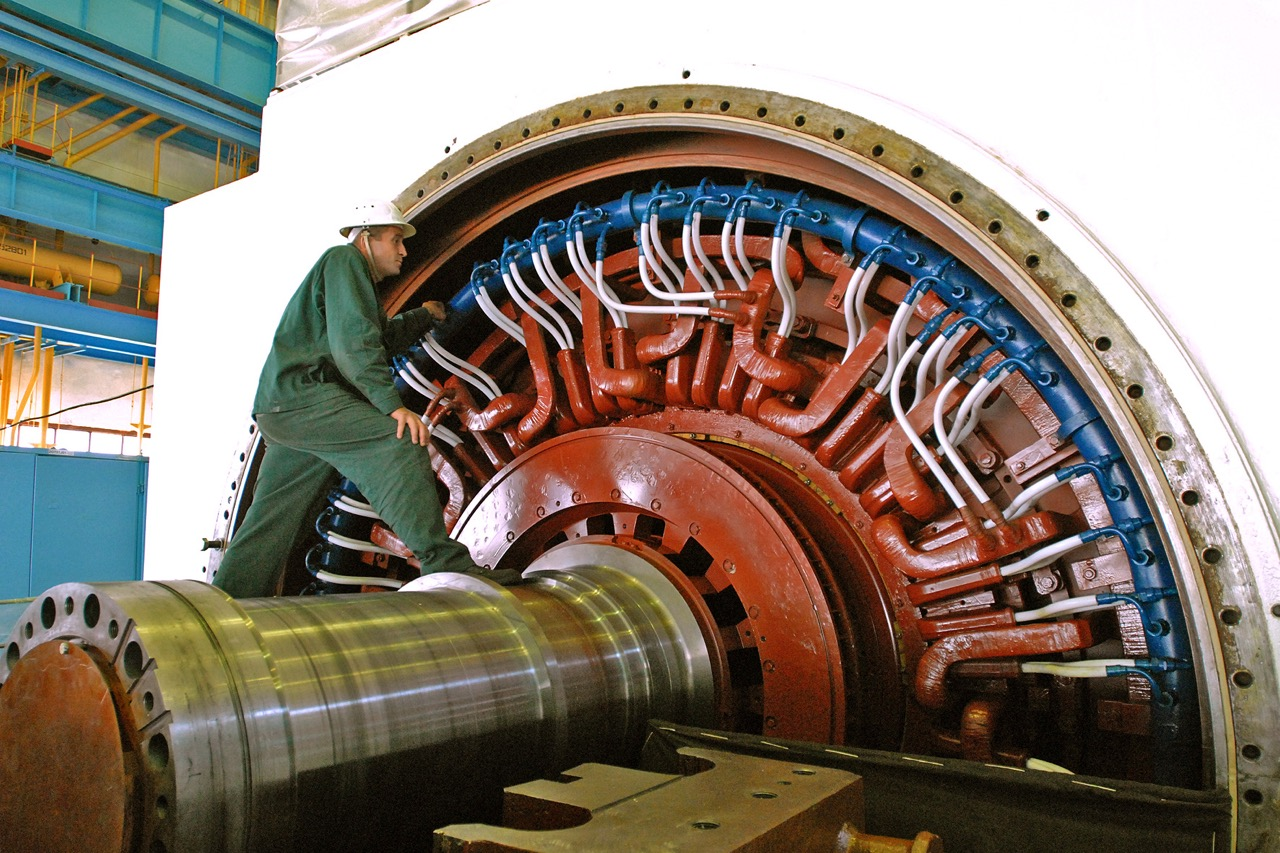
\includegraphics[height=0.55\textheight]{fig/lec07/Turbogenerator_rotor.jpg}
			\caption{\SI[tight-spacing=true]{1}{\giga\volt\ampere} turbogenerator SM rotor from Balakovo nuclear power plant (source: \href{https://commons.wikimedia.org/wiki/File:BalakovoNPP_tb.jpg}{Wikimedia Commons},  A. Seetenky, \href{https://creativecommons.org/licenses/by-sa/3.0/deed}{CC BY-SA 3.0})} 
		\end{subfigure}
        \caption{SM examples with cylindrical rotor type} 
        \label{fig:examples_SM_applications_02}
	\end{figure}
\end{frame}

%%%%%%%%%%%%%%%%%%%%%%%%%%%%%%%%%%%%%%%%%%%%%%%%%%%%%%%%%%%%%
%% Visualization of the synchronous machine operation %%
%%%%%%%%%%%%%%%%%%%%%%%%%%%%%%%%%%%%%%%%%%%%%%%%%%%%%%%%%%%%%
\begin{frame}
	\frametitle{Visualization of the synchronous machine operation}
    \vspace{-0.275cm}
    \begin{figure}
        \centering
        \movie{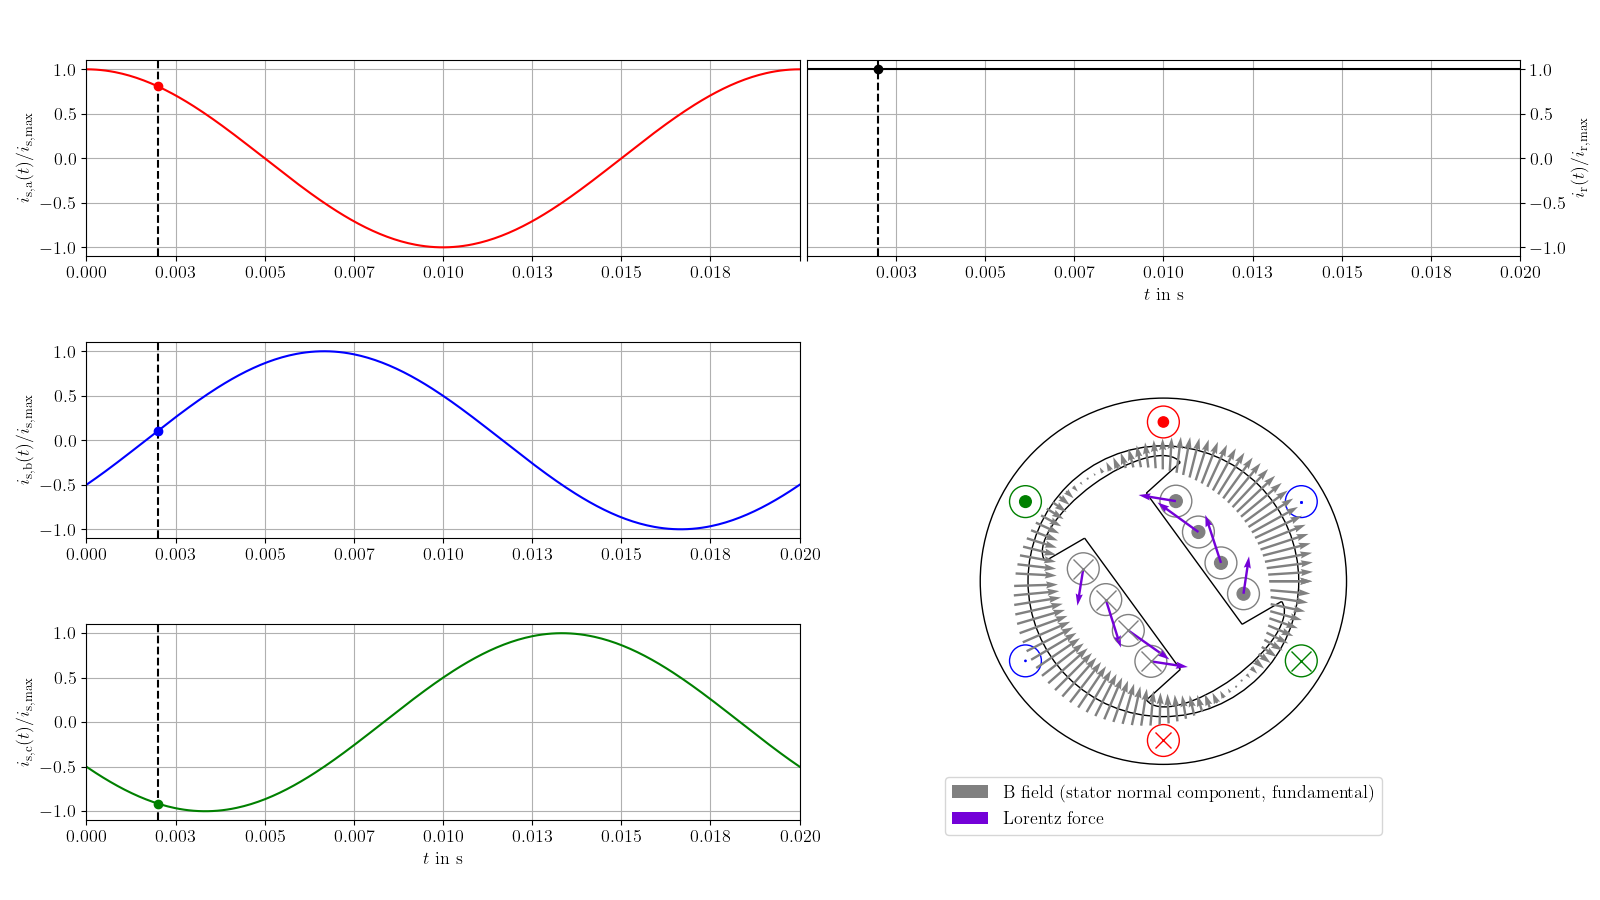
\includegraphics[height=0.85\textheight]{fig/lec07/SM_load_angle_90_preview.png}}{fig/lec07/SM_load_angle_90_animation.gif}
        \vspace{-0.25cm}
        \caption{Exemplary SM operation at $\omega=2 \pi \SI{50}{\per\second}$ in motoric operation (positive average torque)}
        \label{fig:SM_load_angle_90_animation}
    \end{figure}
\end{frame}

%%%%%%%%%%%%%%%%%%%%%%%%%%%%%%%%%%%%%%%%%%%%%%%%%%%%%%%%%%%%%
%% Visualization of the synchronous machine operation (cont.) %%
%%%%%%%%%%%%%%%%%%%%%%%%%%%%%%%%%%%%%%%%%%%%%%%%%%%%%%%%%%%%%
\begin{frame}
	\frametitle{Visualization of the synchronous machine operation (cont.)}
    \vspace{-0.275cm}
    \begin{figure}
        \centering
        \movie{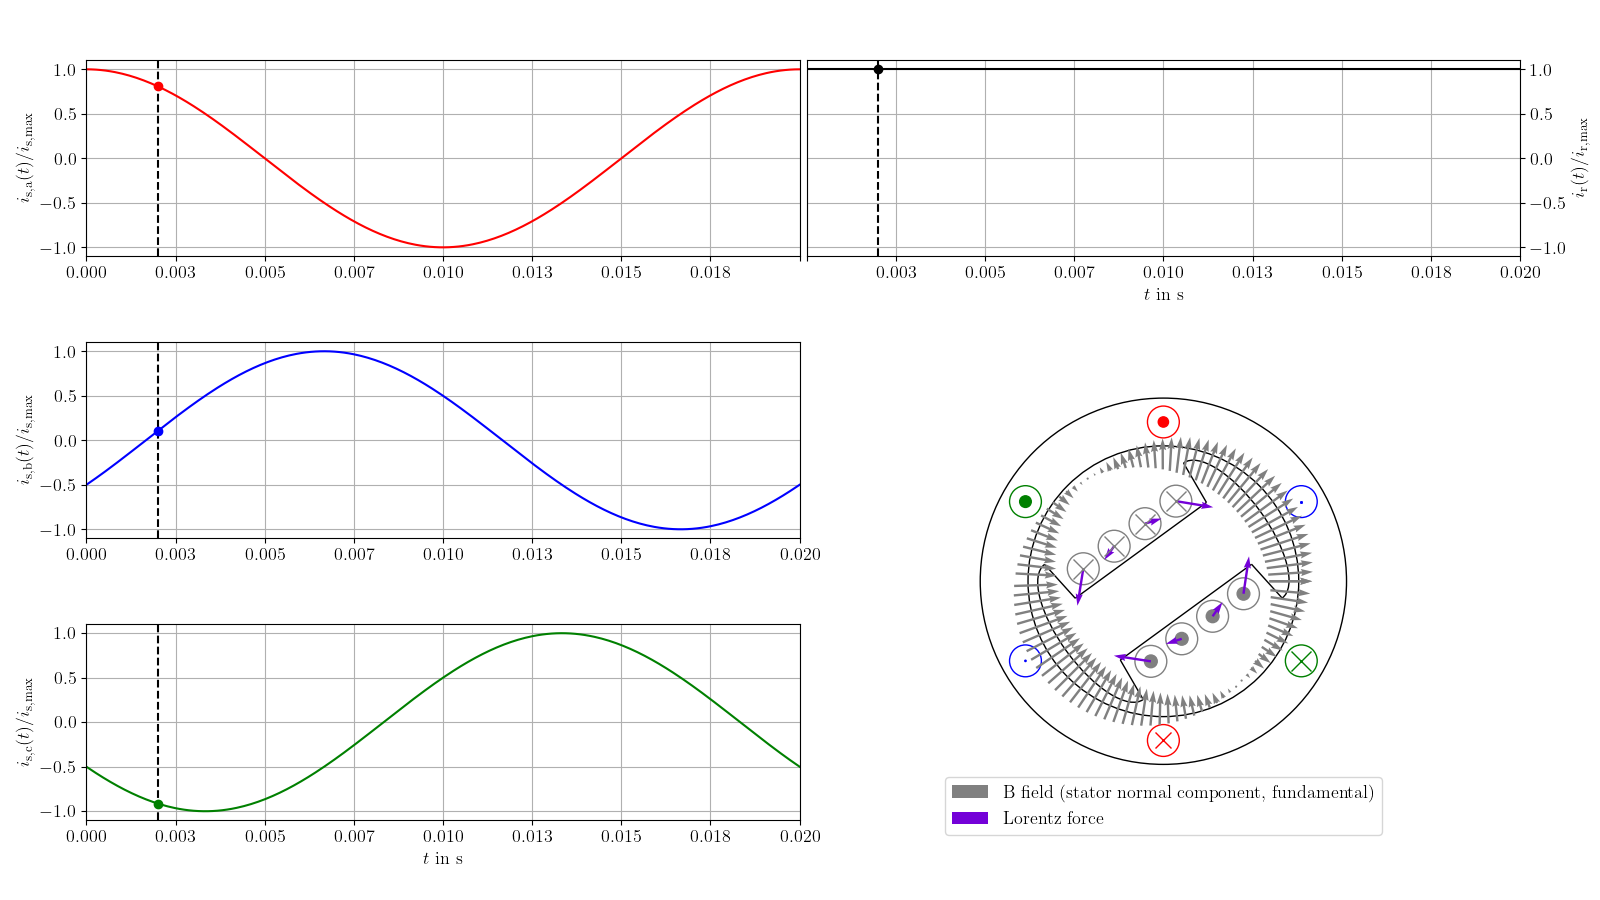
\includegraphics[height=0.85\textheight]{fig/lec07/SM_load_angle_0_preview.png}}{fig/lec07/SM_load_angle_0_animation.gif}
        \vspace{-0.25cm}
        \caption{Exemplary SM operation at $\omega=2 \pi \SI{50}{\per\second}$ in no-load operation (zero average torque)}
        \label{fig:SM_load_angle_0_animation}
    \end{figure}
\end{frame}

%%%%%%%%%%%%%%%%%%%%%%%%%%%%%%%%%%%%%%%%%%%%%%%%%%%%%%%%%%%%%
%% Dynamical IM model %%
%%%%%%%%%%%%%%%%%%%%%%%%%%%%%%%%%%%%%%%%%%%%%%%%%%%%%%%%%%%%%
\begin{frame}
	\frametitle{Dynamical SM model}
    Based on Faraday's and Ohm's laws, we can write the following equations for the stator 
    \begin{equation}
            \bm{u}^\mathrm{s}_\mathrm{s,abc}(t) = R_\mathrm{s}\bm{i}^\mathrm{s}_\mathrm{s,abc}(t)+\frac{\mathrm{d}}{\mathrm{d}t}\bm{\psi}^\mathrm{s}_\mathrm{s,abc}(t) \hspace{0.2cm} \Leftrightarrow \hspace{0.2cm} \begin{bmatrix}
                u_{\mathrm{s,a}}^\mathrm{s}(t)\\
                u_{\mathrm{s,b}}^\mathrm{s}(t)\\
                u_{\mathrm{s,c}}(t)\\
            \end{bmatrix} = R_\mathrm{s} \begin{bmatrix}
                i_{\mathrm{s,a}}^\mathrm{s}(t)\\
                i_{\mathrm{s,b}}^\mathrm{s}(t)\\
                i_{\mathrm{s,c}}^\mathrm{s}(t)\\
            \end{bmatrix} + \frac{\mathrm{d}}{\mathrm{d}t} \begin{bmatrix}
                \psi_{\mathrm{s,a}}^\mathrm{s}(t)\\
                \psi_{\mathrm{s,b}}^\mathrm{s}(t)\\
                \psi_{\mathrm{s,c}}^\mathrm{s}(t)\\
            \end{bmatrix}
            \label{eq:SM_stator_three_phase_voltage_equation}
    \end{equation}
    \pause
    and rotor field windinding
    \begin{equation}
            u^\mathrm{r}_\mathrm{f}(t) = R_\mathrm{f}i^\mathrm{r}_\mathrm{f}(t)+\frac{\mathrm{d}}{\mathrm{d}t}\psi^\mathrm{r}_\mathrm{f}(t) 
            \label{eq:SM_rotor_voltage_equation}
    \end{equation}
which are generally applicable as only identical resistances per phase on the stator are assumed. \pause In contrast to the induction motor, only a single rotor field winding is present.
\end{frame}

%%%%%%%%%%%%%%%%%%%%%%%%%%%%%%%%%%%%%%%%%%%%%%%%%%%%%%%%%%%%%
%% Flux linakge model %%
%%%%%%%%%%%%%%%%%%%%%%%%%%%%%%%%%%%%%%%%%%%%%%%%%%%%%%%%%%%%%
\begin{frame}
	\frametitle{Flux linkage model}
    \onslide<2->
    \begin{columns}
		\begin{column}{0.55\textwidth}
			The SM flux linkage model is similar to the IM model:
	       \begin{itemize}
            \item<2-> Assuming a cylindrical rotor, the self-induced stator flux remains identical to the IM model (derived from rotating field theory chapter).
            \item<3-> In contrast to the IM model \figref{fig:Inductive_coupling_stator_rotor_IM}, the SM's rotor field coil is a represented by a single winding. 
            \item<4-> The coupling of the stator and rotor remains rotor position-dependent (not explicitly shown on the right due to space limitations). 
           \end{itemize}
        \end{column}
        \begin{column}{0.45\textwidth}
            \onslide<1->
                \begin{figure}
                    \centering
                    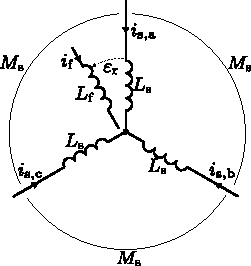
\includegraphics[width=0.75\textwidth]{fig/lec07/Inductive_coupling_stator_rotor.pdf}
                    \caption{Simplified representation of the inductive coupling between the stator/rotor phases of the cylindrical rotor SM}
                    \label{fig:Inductive_coupling_stator_rotor_SM}
                \end{figure}
        \end{column}
    \end{columns}
\end{frame}

%%%%%%%%%%%%%%%%%%%%%%%%%%%%%%%%%%%%%%%%%%%%%%%%%%%%%%%%%%%%%
%% Flux linakge model %%
%%%%%%%%%%%%%%%%%%%%%%%%%%%%%%%%%%%%%%%%%%%%%%%%%%%%%%%%%%%%%
\begin{frame}
	\frametitle{Flux linkages of the three-phase model}
    \onslide<1->
    Based on the previous considerations, the flux linkages of the cylindrical SM are given by
    \begin{equation}
        \renewcommand*{\arraystretch}{1.15}
        \begin{split}
            \uncover<+->{
            \bm{\psi}^\mathrm{s}_\mathrm{s,abc}(t) &=\begin{bmatrix}
                L_\mathrm{s} & -\frac{M_\mathrm{s}}{2} & -\frac{M_\mathrm{s}}{2}\\
                -\frac{M_\mathrm{s}}{2} & L_\mathrm{s} & -\frac{M_\mathrm{s}}{2}\\
                -\frac{M_\mathrm{s}}{2} & -\frac{M_\mathrm{s}}{2} & L_\mathrm{s}
            \end{bmatrix} \bm{i}^\mathrm{s}_\mathrm{s,abc}(t)}\uncover<+->{ +  M_{\mathrm{r}}\frac{N_\mathrm{s}}{N_\mathrm{r}} \begin{bmatrix}
				\cos(\varepsilon_\mathrm{r,el}(t))\\
				 \cos(\varepsilon_\mathrm{r,el}(t) - \frac{2\pi}{3})\\
				 \cos(\varepsilon_\mathrm{r,el}(t) + \frac{2\pi}{3}) 
			 \end{bmatrix}i^\mathrm{r}_\mathrm{f}(t),}\\
            \uncover<+->{
            \psi^\mathrm{r}_\mathrm{f}(t) &= L_\mathrm{f} i^\mathrm{r}_\mathrm{f}(t)\\ &+  M_{\mathrm{s}}\frac{N_\mathrm{r}}{N_\mathrm{s}} \begin{bmatrix}
				\cos(\varepsilon_\mathrm{r,el}(t))  & \cos(\varepsilon_\mathrm{r,el}(t) - \frac{2\pi}{3}) & \cos(\varepsilon_\mathrm{r,el}(t) + \frac{2\pi}{3}) 
			 \end{bmatrix}\bm{i}^\mathrm{s}_\mathrm{s,abc}(t)}
        \end{split}
        \label{eq:Flux_linkage_model_SM_abc}
    \end{equation}
	\onslide<+-> 
    with $\varepsilon_\mathrm{r,el}(t)=p\varepsilon_\mathrm{r}(t)$. \onslide<+-> Consequently, \eqref{eq:Flux_linkage_model_SM_abc} is a reduced representation of the IM's flux linkage model \eqref{eq:Flux_linkage_model_IM_abc}.
\end{frame}

%%%%%%%%%%%%%%%%%%%%%%%%%%%%%%%%%%%%%%%%%%%%%%%%%%%%%%%%%%%%%
%% Cylindrical SM model in alpha-beta coordinates: voltage equations %%
%%%%%%%%%%%%%%%%%%%%%%%%%%%%%%%%%%%%%%%%%%%%%%%%%%%%%%%%%%%%%
\begin{frame}
	\frametitle{Cylindrical SM model in alpha-beta coordinates: voltage equations}
    \begin{columns}
		\begin{column}{0.55\textwidth}
	       Similar to the IM, we can represent the SM model is orthogonal $\alpha\beta$-coordinates. For the SM this only applies to the three-phase stator, as the rotor has only a single phase winding. The $\alpha\beta$-coordinates voltage equation is given by (compare to \eqref{eq:IM_stator_alpha_beta_voltage_equation})
		   \begin{equation}
			\bm{u}^\mathrm{s}_\mathrm{s,\alpha\beta}(t) = R_\mathrm{s} \bm{i}^\mathrm{s}_\mathrm{s,\alpha\beta}(t)+ \frac{\mathrm{d}}{\mathrm{d}t}\bm{\psi}^\mathrm{s}_\mathrm{s,\alpha\beta}(t)
		   \end{equation}
		   \onslide<2->
		   while the rotor field winding voltage equation remains identical to \eqref{eq:SM_rotor_voltage_equation}:
		   $$
			u^\mathrm{r}_\mathrm{f}(t) = R_\mathrm{f}i^\mathrm{r}_\mathrm{f}(t)+\frac{\mathrm{d}}{\mathrm{d}t}\psi^\mathrm{r}_\mathrm{f}(t).
			$$
        \end{column}
        \begin{column}{0.45\textwidth}
            \onslide<1->
            \begin{figure}
                \centering
                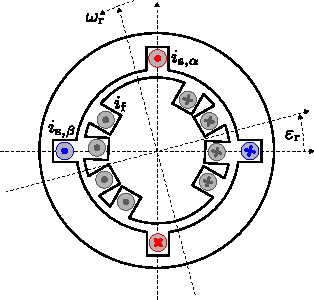
\includegraphics[width=0.85\textwidth]{fig/lec07/SM_cylindrical_rotor_alpha_beta.pdf}
                \caption{Conceptual cylindrical SM representation within the orthogonal $\alpha\beta$ coordinates ($p=1$ pole pair)}
                \label{fig:SM_alpha_beta}
            \end{figure}
        \end{column}
    \end{columns}
\end{frame}


%%%%%%%%%%%%%%%%%%%%%%%%%%%%%%%%%%%%%%%%%%%%%%%%%%%%%%%%%%%%%
%% Cylindrical SM model in alpha-beta coordinates: flux linkage %%
%%%%%%%%%%%%%%%%%%%%%%%%%%%%%%%%%%%%%%%%%%%%%%%%%%%%%%%%%%%%%
\begin{frame}
	\frametitle{Cylindrical SM model in alpha-beta coordinates: flux linkage}
	For the flux linkage model in $\alpha\beta$-coordinates, we multiply the stator flux equations from \eqref{eq:Flux_linkage_model_SM_abc} with $\bm{T}_{23}$ from the right
	\begin{equation}
		\begin{split}
			\bm{\psi}^\mathrm{s}_\mathrm{s,\alpha\beta}(t)  &= \bm{T}_{23} \bm{\psi}^\mathrm{s}_\mathrm{s,abc}(t) = \overbrace{\bm{T}_{23} \bm{L}_{\mathrm{s,abc}}\bm{T}_{32}}^{\bm{L}_{\mathrm{s},\alpha\beta}} \bm{i}^\mathrm{s}_{\mathrm{s},\alpha\beta}(t) +  M_{\mathrm{r}}\frac{N_\mathrm{s}}{N_\mathrm{r}} \bm{T}_{23}\begin{bmatrix}
				\cos(\varepsilon_\mathrm{r,el}(t))\\
				 \cos(\varepsilon_\mathrm{r,el}(t) - \frac{2\pi}{3})\\
				 \cos(\varepsilon_\mathrm{r,el}(t) + \frac{2\pi}{3}) 
			 \end{bmatrix} i^\mathrm{r}_{\mathrm{f}}(t)\\
			 & = (L_\mathrm{s} +\nicefrac{M_\mathrm{s}}{2}) \bm{i}^\mathrm{s}_{\mathrm{s},\alpha\beta}(t) + M_\mathrm{r}\frac{N_\mathrm{s}}{N_\mathrm{r}} \begin{bmatrix}\cos(\varepsilon_\mathrm{r,el}(t))\\ \sin(\varepsilon_\mathrm{r,el}(t))\end{bmatrix} i^\mathrm{r}_{\mathrm{f}}(t)
			\end{split}
	\end{equation}
	and utilize $\bm{i}^\mathrm{s}_\mathrm{s,abc}(t)=\bm{T}_{32} \bm{i}^\mathrm{s}_\mathrm{s,\alpha\beta}(t)$ to modify the rotor flux linkage equation accordingly:
	\begin{equation}
		\begin{split}
			\psi^\mathrm{r}_\mathrm{f}(t) &= L_\mathrm{f} i^\mathrm{r}_\mathrm{f}(t) + M_{\mathrm{s}}\frac{N_\mathrm{r}}{N_\mathrm{s}} \begin{bmatrix}
				\cos(\varepsilon_\mathrm{r,el}(t))  & \sin(\varepsilon_\mathrm{r,el}(t))
			 \end{bmatrix}\bm{i}^\mathrm{s}_\mathrm{s,\alpha\beta}(t).
		\end{split}
	\end{equation} 
	In contrast to the IM $\alpha\beta$-coordinates flux linkage model, the SM flux-to-current coupling is rotor position-dependent.
\end{frame}

%%%%%%%%%%%%%%%%%%%%%%%%%%%%%%%%%%%%%%%%%%%%%%%%%%%%%%%%%%%%%
%% Cylindrical SM model in alpha-beta coordinates: flux linkage (cont.) %%
%%%%%%%%%%%%%%%%%%%%%%%%%%%%%%%%%%%%%%%%%%%%%%%%%%%%%%%%%%%%%
\begin{frame}
	\frametitle{Cylindrical SM model in alpha-beta coordinates: flux linkage (cont.)}
	Analyzing the (magnetic) power balance reveals
    \begin{equation}
        M_\mathrm{r}\frac{N_\mathrm{s}}{N_\mathrm{r}} = M_{\mathrm{s}}\frac{N_\mathrm{r}}{N_\mathrm{s}} \stackrel{!}{=} M_\mathrm{fs}, 
    \end{equation}
    and with the shorter notation 
		\begin{equation}
			L'_\mathrm{s} = (L_\mathrm{s} +\nicefrac{M_\mathrm{s}}{2})
		\end{equation}
	we can rewrite the flux linkage model in $\alpha\beta$-coordinates to
	\begin{equation}
		\begin{alignedat}{2}
			\bm{\psi}^\mathrm{s}_\mathrm{s,\alpha\beta}(t) &= L'_\mathrm{s} \bm{i}^\mathrm{s}_{\mathrm{s},\alpha\beta}(t) &&+ M_\mathrm{fs} \begin{bmatrix}\cos(\varepsilon_\mathrm{r,el}(t))\\ \sin(\varepsilon_\mathrm{r,el}(t))\end{bmatrix} i^\mathrm{r}_{\mathrm{f}}(t),\\
			\psi^\mathrm{r}_\mathrm{f}(t) &= L_\mathrm{f} i^\mathrm{r}_\mathrm{f}(t) &&+ M_\mathrm{fs} \begin{bmatrix}\cos(\varepsilon_\mathrm{r,el}(t)) \\ \sin(\varepsilon_\mathrm{r,el}(t))\end{bmatrix}\T\bm{i}^\mathrm{s}_\mathrm{s,\alpha\beta}(t).
		\end{alignedat}
		\label{eq:Flux_linkage_model_SM_alpha_beta}
	\end{equation}
\end{frame}

%%%%%%%%%%%%%%%%%%%%%%%%%%%%%%%%%%%%%%%%%%%%%%%%%%%%%%%%%%%%%
%% Cylindrical SM model in alpha-beta coordinates: torque %%
%%%%%%%%%%%%%%%%%%%%%%%%%%%%%%%%%%%%%%%%%%%%%%%%%%%%%%%%%%%%%
\begin{frame}
	\frametitle{Cylindrical SM model in alpha-beta coordinates: torque}
	Following the same power balance approach as from the IM, the SM's torque equation is given by
	\begin{equation}
		T(t) = \frac{3}{2} p (\bm{i}_\mathrm{s,\alpha\beta}^\mathrm{s}(t))\T\bm{J}\bm{\psi}_\mathrm{s,\alpha\beta}^\mathrm{s}(t).
	\end{equation}
	The equivalent representation with the rotor current and flux linkage as in the IM case is not applicable in the SM case, as the rotor has only a single field winding, i.e., is lacking an $\alpha\beta$ representation. Inserting the linear flux linkage model from \eqref{eq:Flux_linkage_model_SM_alpha_beta} into the torque equation yields
	\begin{equation}
		\begin{split}
			T(t) &= \frac{3}{2} p (\bm{i}_\mathrm{s,\alpha\beta}^\mathrm{s}(t))\T\bm{J}\bm{\psi}_\mathrm{s,\alpha\beta}^\mathrm{s}(t)\\
			&= \frac{3}{2} p (\bm{i}_\mathrm{s,\alpha\beta}^\mathrm{s}(t))\T\bm{J}\left(L'_\mathrm{s} \bm{i}^\mathrm{s}_{\mathrm{s},\alpha\beta}(t) + M_\mathrm{fs} \begin{bmatrix}\cos(\varepsilon_\mathrm{r,el}(t))\\ \sin(\varepsilon_\mathrm{r,el}(t))\end{bmatrix} i^\mathrm{r}_{\mathrm{f}}(t)\right)\\
			&= \frac{3}{2} p M_\mathrm{fs} i^\mathrm{r}_{\mathrm{f}} \left(\cos(\varepsilon_\mathrm{r,el}(t))i_{\mathrm{s,\beta}}^\mathrm{s}(t) - \sin(\varepsilon_\mathrm{r,el}(t))i_{\mathrm{s,\alpha}}^\mathrm{s}(t)\right).
		\end{split}
		\label{eq:SM_cylindrical_alphabeta_torque_equation}
	\end{equation}
\end{frame}


%%%%%%%%%%%%%%%%%%%%%%%%%%%%%%%%%%%%%%%%%%%%%%%%%%%%%%%%%%%%%
%% Cylindrical SM model in alpha-beta coordinates: voltage equations %%
%%%%%%%%%%%%%%%%%%%%%%%%%%%%%%%%%%%%%%%%%%%%%%%%%%%%%%%%%%%%%
\begin{frame}
	\frametitle{Cylindrical SM model in alpha-beta coordinates: torque interpretation}
    \begin{columns}
		\begin{column}{0.55\textwidth}
			In \eqref{eq:SM_cylindrical_alphabeta_torque_equation} the term
			\begin{equation}
				M_\mathrm{fs} \begin{bmatrix}\cos(\varepsilon_\mathrm{r,el}(t))\\ \sin(\varepsilon_\mathrm{r,el}(t))\end{bmatrix} i^\mathrm{r}_{\mathrm{f}}(t) =\bm{\psi}^\mathrm{s}_{\mathrm{f}}(t)
			\end{equation}
			can be interpreted as the field winding flux linkage coupled with the stator winding. Hence, the torque expression can be rewritten as:
			\begin{equation}
				\begin{split}
				T(t) &= \frac{3}{2} p \left\|\bm{\psi}^\mathrm{s}_{\mathrm{f}}(t) \times \bm{i}^\mathrm{s}_{\mathrm{s,\alpha\beta}}(t)\right\| \\ &= \frac{3}{2} p \left\|\bm{\psi}^\mathrm{s}_{\mathrm{f}}(t) \vphantom{\bm{i}^\mathrm{s}_{\mathrm{s,\alpha\beta}}(t)}\right\| \left\| \bm{i}^\mathrm{s}_{\mathrm{s,\alpha\beta}}(t)\right\| \cos(\theta(t))
			\end{split}
			\end{equation}
			with $\theta$ being the angle between the field winding flux linkage and the stator current vectors, also known as the load angle.
        \end{column}
        \begin{column}{0.45\textwidth}
            \onslide<1->
            \begin{figure}
                \centering
                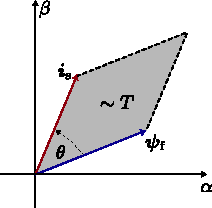
\includegraphics[width=0.75\textwidth]{fig/lec07/Torque_interpretation.pdf}
                \caption{Interpretation of the torque as the parallelogram area spannend by the vectors of the field winding flux and the stator current}
                \label{fig:Torque_interpretation}
            \end{figure}
        \end{column}
    \end{columns}
\end{frame}

%%%%%%%%%%%%%%%%%%%%%%%%%%%%%%%%%%%%%%%%%%%%%%%%%%%%%%%%%%%%%
%% Summary: Cylindrical SM model in $\alpha\beta$ coordinates   %%
%%%%%%%%%%%%%%%%%%%%%%%%%%%%%%%%%%%%%%%%%%%%%%%%%%%%%%%%%%%%%
\begin{frame}
	\frametitle{Summary: Cylindrical SM model in $\alpha\beta$ coordinates}
    The most important equations of the cylindrical SM model in the  $\alpha\beta$ coordinates are:
    \begin{equation*}
        \begin{alignedat}{4}
            &&\mbox{Stator voltage:}&& \quad\bm{u}^\mathrm{s}_\mathrm{s,\alpha\beta}(&t) &&= R_\mathrm{s} \bm{i}^\mathrm{s}_\mathrm{s,\alpha\beta}(t)+ \frac{\mathrm{d}}{\mathrm{d}t}\bm{\psi}^\mathrm{s}_\mathrm{s,\alpha\beta}(t),\\
            &&\mbox{Rotor / field winding voltage:}&& \quad u^\mathrm{r}_\mathrm{f}(&t) &&= R_\mathrm{f}i^\mathrm{r}_\mathrm{f}(t)+\frac{\mathrm{d}}{\mathrm{d}t}\psi^\mathrm{r}_\mathrm{f}(t),\\
            &&\mbox{Stator flux linkage:}&& \quad \bm{\psi}^\mathrm{s}_\mathrm{s,\alpha\beta}(&t) &&= L'_\mathrm{s} \bm{i}^\mathrm{s}_{\mathrm{s},\alpha\beta}(t) + M_\mathrm{fs} \begin{bmatrix}\cos(\varepsilon_\mathrm{r,el}(t))\\ \sin(\varepsilon_\mathrm{r,el}(t))\end{bmatrix} i^\mathrm{r}_{\mathrm{f}}(t),\\
            &&\mbox{Rotor / field winding flux linkage:}&& \psi^\mathrm{r}_\mathrm{f}(&t) &&= L_\mathrm{f} i^\mathrm{r}_\mathrm{f}(t) + M_\mathrm{fs} \begin{bmatrix}\cos(\varepsilon_\mathrm{r,el}(t)) \\ \sin(\varepsilon_\mathrm{r,el}(t))\end{bmatrix}\T\bm{i}^\mathrm{s}_\mathrm{s,\alpha\beta}(t),\\
            &&\mbox{Torque:}&& \quad T(&t) &&= \frac{3}{2} p (\bm{i}_\mathrm{s,\alpha\beta}^\mathrm{s})\T\bm{J}\bm{\psi}_\mathrm{s,\alpha\beta}^\mathrm{s}. 
        \end{alignedat}
    \end{equation*}
\end{frame}

%%%%%%%%%%%%%%%%%%%%%%%%%%%%%%%%%%%%%%%%%%%%%%%%%%%%%%%%%%%%%
%% Rotor flux orientation: the dq coordinate system %%
%%%%%%%%%%%%%%%%%%%%%%%%%%%%%%%%%%%%%%%%%%%%%%%%%%%%%%%%%%%%%
\begin{frame}
	\frametitle{Rotor flux orientation: the dq coordinate system}	
    \begin{columns}
		\begin{column}{0.5\textwidth}
			\begin{itemize}
				\item In the SM case the rotor flux orientaton is directly related to the rotor position (cf. \figref{fig:examples_SM_rotor}). 
				\item Hence, to transfer the rotor and stator equations into a mutual coordinate system, the rotor flux orientation is typically used as a reference. 
				\item In contrast to the $\alpha\beta$-coordinates, where the stator quantity signals are of sinusoidal shape during steady state, the rotor flux-oriented signals are constant during steady state.
			\end{itemize}
		\end{column}
        \begin{column}{0.5\textwidth}
            \begin{figure}
                \centering
                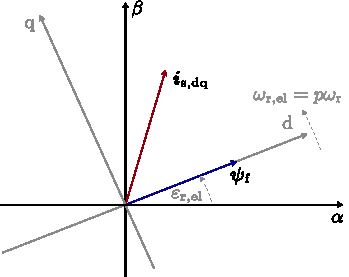
\includegraphics[width=0.9\textwidth]{fig/lec07/dq_orientation.pdf}
                \caption{Rotor flux-oriented coordinate system}
                \label{fig:dq_orientation}
            \end{figure}
        \end{column}
    \end{columns}
\end{frame}

%%%%%%%%%%%%%%%%%%%%%%%%%%%%%%%%%%%%%%%%%%%%%%%%%%%%%%%%%%%%%
%% Rotor flux orientation: the dq coordinate system (cont.) %%
%%%%%%%%%%%%%%%%%%%%%%%%%%%%%%%%%%%%%%%%%%%%%%%%%%%%%%%%%%%%%
\begin{frame}
	\frametitle{Rotor flux orientation: the dq coordinate system (cont.) }
	Transferring the stator voltage equation into the dq coordinate system results in
		   \begin{equation}
			\begin{split}
			\bm{u}^\mathrm{s}_\mathrm{s,\alpha\beta}(t) &= R_\mathrm{s} \bm{i}^\mathrm{s}_\mathrm{s,\alpha\beta}(t)+ \frac{\mathrm{d}}{\mathrm{d}t}\bm{\psi}^\mathrm{s}_\mathrm{s,\alpha\beta}(t)\\
			\Leftrightarrow \quad \bm{T}^{-1}_\mathrm{p}(\varepsilon_\mathrm{r,el})\bm{u}^\mathrm{s}_\mathrm{s,dq}(t) &= R_\mathrm{s} \bm{T}^{-1}_\mathrm{p}(\varepsilon_\mathrm{r,el})\bm{i}^\mathrm{s}_\mathrm{s,dq}(t)+ \frac{\mathrm{d}}{\mathrm{d}t}(\bm{T}^{-1}_\mathrm{p}(\varepsilon_\mathrm{r,el})\bm{\psi}^\mathrm{s}_\mathrm{s,dq}(t))\\
			\Leftrightarrow \quad \bm{u}^\mathrm{r}_\mathrm{s,dq}(t) &= R_\mathrm{s} \bm{i}^\mathrm{r}_\mathrm{s,dq}(t)+ \omega_\mathrm{r,el}(t)\bm{J}\bm{\psi}^\mathrm{r}_\mathrm{s,dq}(t) + \frac{\mathrm{d}}{\mathrm{d}t}\bm{\psi}^\mathrm{r}_\mathrm{s,dq}(t).
		\end{split}
		\end{equation}
	Since the dq coordinate system is always aligned with the rotor flux in the SM case, one can also drop the superscript $r$:
	\begin{equation*}
		\bm{u}_\mathrm{s,dq}(t) = R_\mathrm{s} \bm{i}_\mathrm{s,dq}(t)+ \omega_\mathrm{r,el}(t)\bm{J}\bm{\psi}_\mathrm{s,dq}(t) + \frac{\mathrm{d}}{\mathrm{d}t}\bm{\psi}_\mathrm{s,dq}(t).
	\end{equation*} 
\end{frame}

%%%%%%%%%%%%%%%%%%%%%%%%%%%%%%%%%%%%%%%%%%%%%%%%%%%%%%%%%%%%%
%% Rotor flux orientation: the dq coordinate system (cont.) %%
%%%%%%%%%%%%%%%%%%%%%%%%%%%%%%%%%%%%%%%%%%%%%%%%%%%%%%%%%%%%%
\begin{frame}
	\frametitle{Rotor flux orientation: the dq coordinate system (cont.) }
	The stator flux linkage model in the dq coordinate system is given by
	\begin{equation}
		\begin{split}
			\bm{\psi}^\mathrm{s}_\mathrm{s,\alpha\beta}(t) &= L'_\mathrm{s} \bm{i}^\mathrm{s}_{\mathrm{s},\alpha\beta}(t) + M_\mathrm{fs} \begin{bmatrix}\cos(\varepsilon_\mathrm{r,el}(t))\\ \sin(\varepsilon_\mathrm{r,el}(t))\end{bmatrix} i^\mathrm{r}_{\mathrm{f}}(t),			 \\ \Leftrightarrow \quad 
			 \bm{T}^{-1}_\mathrm{p}(\varepsilon_\mathrm{r,el}) \bm{\psi}_\mathrm{s,dq}(t) &= L'_\mathrm{s}  \bm{T}^{-1}_\mathrm{p}(\varepsilon_\mathrm{r,el})\bm{i}_{\mathrm{s, dq}}(t) + M_\mathrm{fs} \begin{bmatrix}\cos(\varepsilon_\mathrm{r,el}(t)) \\ \sin(\varepsilon_\mathrm{r,el}(t))\end{bmatrix}i_{\mathrm{f}}(t) \\
			 \Leftrightarrow \quad \bm{\psi}_\mathrm{s,dq}(t) &= L'_\mathrm{s} \bm{i}_{\mathrm{s,dq}}(t) + M_\mathrm{fs} \begin{bmatrix}1 \\ 0 \end{bmatrix}i^\mathrm{r}_{\mathrm{f}}(t).
		\end{split}
		\label{eq:SM_stator_dq_flux_linkage}
	\end{equation}
	while the field winding flux results in
	\begin{equation}
		\begin{split}
             \psi^\mathrm{r}_\mathrm{f}(t) &= L_\mathrm{f} i^\mathrm{r}_\mathrm{f}(t) + M_\mathrm{fs} \begin{bmatrix}\cos(\varepsilon_\mathrm{r,el}(t)) & \sin(\varepsilon_\mathrm{r,el}(t))\end{bmatrix}\bm{i}^\mathrm{s}_\mathrm{s,\alpha\beta}(t)
			 \\ \Leftrightarrow \quad 	 \psi^\mathrm{r}_\mathrm{f}(t) &= L_\mathrm{f} i^\mathrm{r}_\mathrm{f}(t) + M_\mathrm{fs} \begin{bmatrix}\cos(\varepsilon_\mathrm{r,el}(t)) & \sin(\varepsilon_\mathrm{r,el}(t))\end{bmatrix}  \bm{T}^{-1}_\mathrm{p}(\varepsilon_\mathrm{r,el})\bm{i}^\mathrm{s}_\mathrm{s,dq}(t)
			 \\
			 \Leftrightarrow \quad \psi^\mathrm{r}_\mathrm{f}(t) &= L_\mathrm{f} i^\mathrm{r}_\mathrm{f}(t) + M_\mathrm{fs} \begin{bmatrix}1 & 0\end{bmatrix} \bm{i}_\mathrm{s,dq}(t).
		\end{split}
	\end{equation}
\end{frame}

%%%%%%%%%%%%%%%%%%%%%%%%%%%%%%%%%%%%%%%%%%%%%%%%%%%%%%%%%%%%%
%% Summary: Cylindrical SM model in dq coordinates   %%
%%%%%%%%%%%%%%%%%%%%%%%%%%%%%%%%%%%%%%%%%%%%%%%%%%%%%%%%%%%%%
\begin{frame}
	\frametitle{Summary: Cylindrical SM model in dq coordinates}
    The most important equations of the cylindrical SM model in the  dq coordinates are:
    \begin{equation*}
        \begin{alignedat}{4}
            &&\mbox{Stator voltage:}&& \quad\bm{u}_\mathrm{s,dq}(&t) &&= R_\mathrm{s} \bm{i}_\mathrm{s,dq}(t)+ \omega_\mathrm{r,el}(t)\bm{J}\bm{\psi}_\mathrm{s,dq}(t) + \frac{\mathrm{d}}{\mathrm{d}t}\bm{\psi}_\mathrm{s,dq}(t),\\
			&&\mbox{Rotor / field winding  voltage:}&& \quad u_\mathrm{f}(&t) &&= R_\mathrm{f}i_\mathrm{f}(t)+\frac{\mathrm{d}}{\mathrm{d}t}\psi_\mathrm{f}(t),\\
			&&\mbox{Stator flux linkage:}&& \quad \bm{\psi}_\mathrm{s,dq}(&t) &&= L'_\mathrm{s} \bm{i}_\mathrm{s,dq}(t) + M_\mathrm{fs} \begin{bmatrix}1 \\ 0\end{bmatrix} i_{\mathrm{f}}(t),\\
			&&\mbox{Rotor / field winding flux linkage:}&& \psi_\mathrm{f}(&t) &&= L_\mathrm{f} i^\mathrm{r}_\mathrm{f}(t) + M_\mathrm{fs} \begin{bmatrix}1 & 0\end{bmatrix} \bm{i}_\mathrm{s,dq}(t),\\
			&&\mbox{Torque:}&& \quad T(&t) &&= \frac{3}{2} p (\bm{i}_\mathrm{s,dq})\T\bm{J}\bm{\psi}_\mathrm{s,dq}.
        \end{alignedat}
    \end{equation*}
	Here, one can observe that the d component of the stator flux linkage is directly coupled with the field winding flux and vice versa, which was to be expected due to the rotor flux orientation of the chosen coordinate system.  
\end{frame}

%%%%%%%%%%%%%%%%%%%%%%%%%%%%%%%%%%%%%%%%%%%%%%%%%%%%%%%%%%%%%
%% Salient pole SM model %%
%%%%%%%%%%%%%%%%%%%%%%%%%%%%%%%%%%%%%%%%%%%%%%%%%%%%%%%%%%%%%
\begin{frame}
	\frametitle{Salient pole SM model}	
    \begin{columns}
		\begin{column}{0.5\textwidth}
			\begin{itemize}
				\item The cylindrical rotor SM model \eqref{eq:SM_stator_dq_flux_linkage} considered an identical stator inductance $L'_\mathrm{s}$ for the d and q axis.  
				\item In the cylindrical SM case this is a valid assumption, as the rotor is symmetrical. 
				\item However, in the case of a salient pole SM, the rotor is not symmetrical and the flux path per axis is different (cf. \figref{fig:SM_salient_pole_dq_reluctance}).
				\item The q-axis reluctance is larger than the d-axis reluctance due to the larger air gap in the q-axis direction. 
				\item Consequently, the inductance per axis is different.
			\end{itemize}
		\end{column}
        \begin{column}{0.5\textwidth}
            \begin{figure}
                \centering
                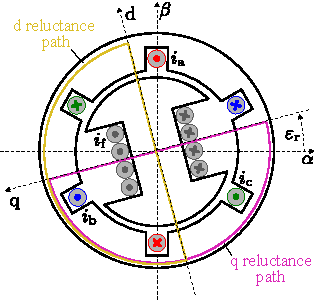
\includegraphics[width=0.825\textwidth]{fig/lec07/SM_salient_pole_dq_reluctance.pdf}
                \caption{Effective reluctance paths of the salient pole SM in the dq coordinate system}
                \label{fig:SM_salient_pole_dq_reluctance}
            \end{figure}
        \end{column}
    \end{columns}
\end{frame}